\documentclass[zihao=false,fontset=windows]{ctexart}
% ctexart 不接受任意 pt 选项。正文改 {10pt}，方括号里是行距。
\usepackage{scrextend}
\changefontsizes[12pt]{10pt}

\usepackage[a4paper,left=2.35cm,right=2.35cm,top=1.7cm,bottom=1.9cm]{geometry}
\usepackage{xcolor}
\usepackage{graphicx}
\usepackage{amsmath,amssymb}
\usepackage{enumitem}
\usepackage{tabularx}
\usepackage{colortbl}
\usepackage{listings}
\usepackage{hyperref}
\usepackage[most]{tcolorbox}

\definecolor{feishuText}{RGB}{31,35,41}
\definecolor{feishuBlue}{RGB}{36,91,219}
\definecolor{feishuRed}{RGB}{216,57,49}
\definecolor{feishuGray}{RGB}{100,106,115}
\definecolor{feishuGray2}{RGB}{143,149,158}
\definecolor{feishuPinkBg}{RGB}{251,191,188}
\definecolor{quoteBar}{RGB}{51,112,255}
\definecolor{codebg}{RGB}{245,246,247}
\definecolor{codeborder}{RGB}{222,224,227}
\definecolor{inlinebg}{RGB}{242,243,245}
\definecolor{callRed}{RGB}{253,226,226}
\definecolor{callOrange}{RGB}{255,245,235}
\definecolor{callYellow}{RGB}{254,255,240}
\definecolor{callGreen}{RGB}{240,251,239}
\definecolor{callBlue}{RGB}{240,244,255}
\definecolor{callRedSoft}{RGB}{254,241,241}
\definecolor{callSun}{RGB}{255,255,204}
\definecolor{tableHead}{RGB}{242,243,245}
\definecolor{tableRule}{RGB}{222,224,227}
\definecolor{codeText}{RGB}{31,35,41}
\definecolor{codeKeyword}{RGB}{0,0,255}
\definecolor{codeComment}{RGB}{0,128,0}
\definecolor{codeString}{RGB}{163,21,21}

\setmainfont{Times New Roman}
\setCJKmainfont{Microsoft YaHei}[AutoFakeBold=2.2]
\setCJKsansfont{Microsoft YaHei}[AutoFakeBold=2.2]
\setCJKmonofont{Microsoft YaHei}[AutoFakeBold=2.2]
\setmonofont{Consolas}
\newfontfamily\emojifont{Segoe UI Emoji}

\hypersetup{
  colorlinks=true,
  urlcolor=feishuBlue,
  linkcolor=feishuBlue,
  unicode=true,
  pdftitle={mPLUG-OWL(2023, Alibaba)}
}

\setlength{\parindent}{0pt}
\setlength{\parskip}{0.42em}
\setlength{\fboxsep}{1.5pt}
\setlength{\emergencystretch}{3em}
\linespread{1.28}
\color{feishuText}
\arrayrulecolor{tableRule}
\urlstyle{same}

\setlist[enumerate]{label=\textcolor{feishuBlue}{\arabic*.}, leftmargin=1.7em, itemsep=0.22em, topsep=0.28em, parsep=0.08em, partopsep=0pt}
\setlist[itemize,1]{label=\textcolor{feishuBlue}{\textbullet}, leftmargin=1.35em, itemsep=0.18em, topsep=0.25em, parsep=0.06em, partopsep=0pt}
\setlist[itemize,2]{label=\textcolor{feishuBlue}{◦}, leftmargin=1.45em, itemsep=0.12em, topsep=0.15em}
\setlist[itemize,3]{label=\textcolor{feishuBlue}{\rule[0.18em]{0.38em}{0.38em}}, leftmargin=1.55em, itemsep=0.1em, topsep=0.12em}

\newcommand{\feiEmoji}[1]{{\emojifont #1}}
\newcommand{\incode}[1]{\colorbox{inlinebg}{\ttfamily\small #1}}
\newcommand{\bigmath}[1]{%
  \begin{center}\large$\displaystyle #1$\end{center}%
}

\lstset{
  language=Python,
  basicstyle=\ttfamily\footnotesize\color{codeText},
  keywordstyle=\color{codeKeyword},
  commentstyle=\color{codeComment},
  stringstyle=\color{codeString},
  showstringspaces=false,
  breaklines=true,
  columns=fullflexible,
  keepspaces=true,
  tabsize=4,
  upquote=true,
  aboveskip=2pt,
  belowskip=0pt,
  xleftmargin=0pt,
  frame=none
}

\tcbset{
  feishubase/.style 2 args={
    enhanced,
    boxrule=0pt,
    arc=8pt,
    left=10pt,
    right=10pt,
    top=7pt,
    bottom=7pt,
    before skip=6pt,
    after skip=6pt,
    colback=#1,
    colframe=#1,
    before upper={\feiEmoji{#2}\hspace{0.45em}\ignorespaces}
  }
}
\newtcolorbox{feishubox}[2]{feishubase={#1}{#2}, breakable}
\newtcolorbox{feishuboxnb}[2]{feishubase={#1}{#2}}

\newtcolorbox{feishuquote}{
  enhanced,
  breakable,
  boxrule=0pt,
  leftrule=3pt,
  arc=0pt,
  colframe=quoteBar,
  colback=white,
  left=8pt,
  right=2pt,
  top=2pt,
  bottom=2pt,
  before skip=4pt,
  after skip=4pt,
  before upper=\color{feishuGray}
}

\newtcolorbox{feishucode}{
  enhanced,
  breakable,
  colback=codebg,
  colframe=codeborder,
  boxrule=0.6pt,
  arc=6pt,
  left=6pt,
  right=6pt,
  top=5pt,
  bottom=4pt,
  before skip=6pt,
  after skip=6pt
}

% Source: https://scnajei2ds6y.feishu.cn/wiki/SEDGwBr2TimSUpkTkOlclwfSn5f
% Faithful reproduction of Feishu body; excludes cover, AI summary, back-reference UI.
% Figures: screenshots of the normal image preview, cropped locally (1216x578 / 1216x360).
\begin{document}
{\zihao{1}\bfseries mPLUG-OWL(2023, Alibaba)\par}

\begin{feishubox}{callOrange}{🙋‍♀}
论文：《\textcolor{feishuGray}{mPLUG-Owl: Modularization Empowers Large Language Models with Multimodality》}\par
论文地址：\url{https://arxiv.org/pdf/2304.14178}\par
项目地址：\url{https://github.com/X-PLUG/mPLUG-Owl}\par
\end{feishubox}

\par\vspace{1.15em}\noindent{\zihao{-2}\bfseries \textcolor{feishuBlue}{1.} 模型结构}\par\vspace{0.28em}
\begin{center}
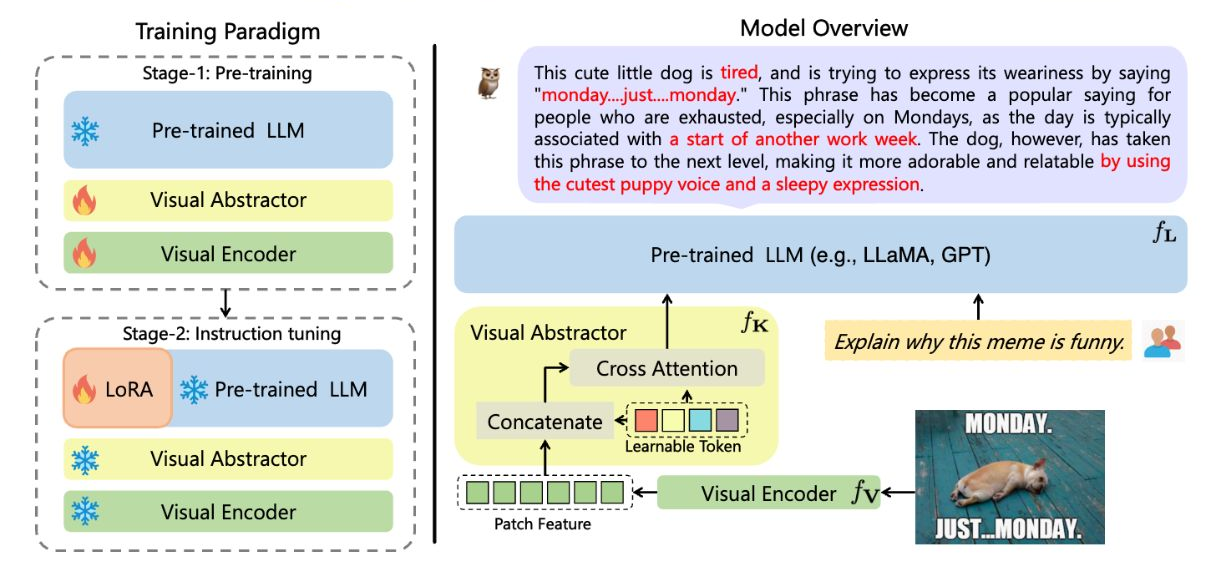
\includegraphics[width=0.98\textwidth]{images/2023-mPLUG-OWL/fig-01.png}
\end{center}
mPLUG-owl已经和最新(2025年)的mllm结构基本一致了，也是分为三个模块：\par

\par\vspace{0.95em}\noindent{\zihao{3}\bfseries \textcolor{feishuBlue}{1.1} Visual Encoder}\par\vspace{0.28em}
使用的是ViT-L/14（num\_layers = 24，hidden\_dimension=1024，patch\_size=14）。\par
参数量大约0.2B。\par

\par\vspace{0.95em}\noindent{\zihao{3}\bfseries \textcolor{feishuBlue}{1.2} LLM}\par\vspace{0.28em}
LLaMA-7B pretrain版本。\par

\par\vspace{0.95em}\noindent{\zihao{3}\bfseries \textcolor{feishuBlue}{1.3} Adapter（Visual Abstractor）}\par\vspace{0.28em}
这个结构参考的是\href{https://scnajei2ds6y.feishu.cn/wiki/Cb61wEeXDi5NQSkARrbcu8PynEf}{Flamingo(2022, DeepMind)}的Resampler，虽然\href{https://scnajei2ds6y.feishu.cn/wiki/AZiVwFmXEirI77kAVzYcOMNVnbh}{BLIP-2(2023, Salesforce Research)}也使用 类似Learnable Token的技术，但是有一个细节，mPLUG和\href{https://scnajei2ds6y.feishu.cn/wiki/Cb61wEeXDi5NQSkARrbcu8PynEf}{Flamingo(2022, DeepMind)}的Resampler会讲Learnable Token拼接到视觉KV中去。\par

\begin{feishucode}
\begin{lstlisting}
class MplugOwlVisualAbstractorAttention(nn.Module):
    def __init__(self, config: MplugOwlVisualAbstractorConfig):
        super().__init__()
        self.attention = MplugOwlVisualAbstractorMultiHeadAttention(config)
        self.output = MplugOwlVisualAbstractorCrossOutput(config)
        self.pruned_heads = set()
        self.norm1 = LayerNormFp32(config.hidden_size)
        self.normk = LayerNormFp32(config.hidden_size)

    def prune_heads(self, heads):
        if len(heads) == 0:
            return
        heads, index = find_pruneable_heads_and_indices(
            heads, self.attention.num_attention_heads, self.attention.attention_head_size, self.pruned_heads
        )

        # Prune linear layers
        self.attention.query = prune_linear_layer(self.attention.query, index)
        self.attention.key = prune_linear_layer(self.attention.key, index)
        self.attention.value = prune_linear_layer(self.attention.value, index)
        self.output.dense = prune_linear_layer(self.output.out_proj, index, dim=1)

        # Update hyper params and store pruned heads
        self.attention.num_attention_heads = self.attention.num_attention_heads - len(heads)
        self.attention.all_head_size = self.attention.attention_head_size * self.attention.num_attention_heads
        self.pruned_heads = self.pruned_heads.union(heads)

    def forward(
        self,
        hidden_states: torch.Tensor,
        attention_mask: Optional[torch.FloatTensor] = None,
        head_mask: Optional[torch.FloatTensor] = None,
        encoder_hidden_states: Optional[torch.FloatTensor] = None,
        encoder_attention_mask: Optional[torch.FloatTensor] = None,
        past_key_value: Optional[Tuple[Tuple[torch.FloatTensor]]] = None,
        output_attentions: Optional[bool] = False,
    ) -> Tuple[torch.Tensor]:
        # HACK we apply norm on q and k
        hidden_states = self.norm1(hidden_states)
        encoder_hidden_states = self.normk(encoder_hidden_states)
        encoder_hidden_states = torch.cat([hidden_states, encoder_hidden_states], dim=1)
        encoder_attention_mask = torch.cat([attention_mask, encoder_attention_mask], dim=-1)
        self_outputs = self.attention(
            hidden_states,
            attention_mask,
            head_mask,
            encoder_hidden_states,
            encoder_attention_mask,
            past_key_value,
            output_attentions,
        )
        attention_output = self.output(self_outputs[0], hidden_states)
        # add attentions if we output them
        outputs = (attention_output,) + self_outputs[1:]
        return outputs
\end{lstlisting}
\end{feishucode}

\clearpage
\par\vspace{1.15em}\noindent{\zihao{-2}\bfseries \textcolor{feishuBlue}{2.} 训练}\par\vspace{0.28em}
下面这张图很好的展示了mPLUG-OWL和一些同期模型的训练区别。\par
\begin{center}
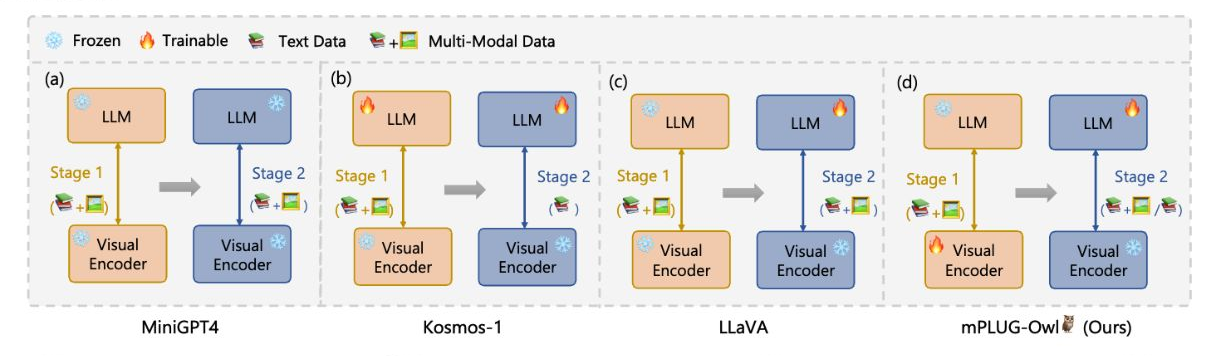
\includegraphics[width=0.98\textwidth]{images/2023-mPLUG-OWL/fig-02.png}
\end{center}

\par\vspace{0.95em}\noindent{\zihao{3}\bfseries \textcolor{feishuBlue}{2.1} Stage 1}\par\vspace{0.28em}
使用的数据格式是image-caption pairs，采样于 LAION-400M、COYO-700M、Conceptual Caption、MSCOCO。\par
使用了批量大小为 2.1 million 个 token，并将 mPLUG-Owl 训练 50k 步，对应大约 104 billion个 token。我们采用 AdamW 优化器，β 参数设为 (0.9, 0.98)，学习率和权重衰减系数分别设置为 0.0001 和 0.1。训练初期先进行 2000 步的学习率预热（warm-up），然后采用余弦退火（cosine schedule）来衰减学习率。输入图像会被随机调整为 224 × 224 的尺寸。\par
文本编码器使用的是  SentencePiece。\par

\par\vspace{0.95em}\noindent{\zihao{3}\bfseries \textcolor{feishuBlue}{2.2} Stage 2}\par\vspace{0.28em}
在第二阶段，从三个不同来源收集了纯文本指令数据，102k data from the Alpaca、90k from the Vicuna和 50k from the Baize。此外，我们还使用了来自 LLaVA 数据集的 50k 条多模态指令数据。\par
对 mPLUG-Owl 进行 2000 步训练，批量大小为 256，学习率设为 2*10\textasciicircum{}-5。\par
\end{document}
